
\section{仿真测试}

本次实验使用 Vivado 2017.3 进行仿真测试。

\subsection{Hamming 编解码}

仿真文件如下:
\begin{codeblock}{verilog}
`define PERIOD 10
module hamming_tb();
    reg [3:0] data_i;
    wire [6:0] data_enc;
    wire [3:0] data_dec;
    hamming_encode hamming_encode_0 (
        .data_i(data_i),
        .data_o(data_enc)
    );
    hamming_decode hamming_decode_0 (
        .data_i(data_enc),
        .data_o(data_dec)
    );
    integer i;
    initial begin
        for (i = 0; i < 16; i=i+1) begin
            data_i = i;
            #(`PERIOD)
            if (data_dec ! = data_i) begin
                $display("[Error]: %b -> %b -> %b", data_i, data_enc, data_dec);
            end 
            else begin
                $display("Correct: %b -> %b -> %b", data_i, data_enc, data_dec);
            end
        end
    end
endmodule
\end{codeblock}

输出如下:
\begin{codeblock}{verilog}
Correct: 0000 -> 0000000 -> 0000
Correct: 0001 -> 1110001 -> 0001
Correct: 0010 -> 1010010 -> 0010
Correct: 0011 -> 0100011 -> 0011
Correct: 0100 -> 0110100 -> 0100
Correct: 0101 -> 1000101 -> 0101
Correct: 0110 -> 1100110 -> 0110
Correct: 0111 -> 0010111 -> 0111
Correct: 1000 -> 1101000 -> 1000
Correct: 1001 -> 0011001 -> 1001
Correct: 1010 -> 0111010 -> 1010
Correct: 1011 -> 1001011 -> 1011
Correct: 1100 -> 1011100 -> 1100
Correct: 1101 -> 0101101 -> 1101
Correct: 1110 -> 0001110 -> 1110
Correct: 1111 -> 1111111 -> 1111
\end{codeblock}

这表明 Hamming 码编解码模块实现正确。

\subsection{交织与解交织}

仿真文件如下:
\begin{codeblock}{verilog}
module test_IL();  
    reg clk;
    reg rst;
    reg en;
    reg [28 -1:0] data = 28'b0011111000011110110111100101;
    wire en_IL;
    wire [28 -1:0] data_IL;
    interleaver il(clk, rst, en, data, en_IL, data_IL);
    wire [28 -1:0] data_DIL;
    wire en_DIL;
    deinterleaver dil(clk, rst, en_IL, data_IL, en_DIL, data_DIL);
    initial begin
        clk <= 1;
        rst <= 0;
        en <= 0;
        #10 en <= 1;
        rst <= 1;
    end
    always #5 clk = ~clk; 
endmodule
\end{codeblock}

仿真结果如图 \ref{fig:interleave_simulation1} 所示。

\begin{figure}[ht]
    \centering
    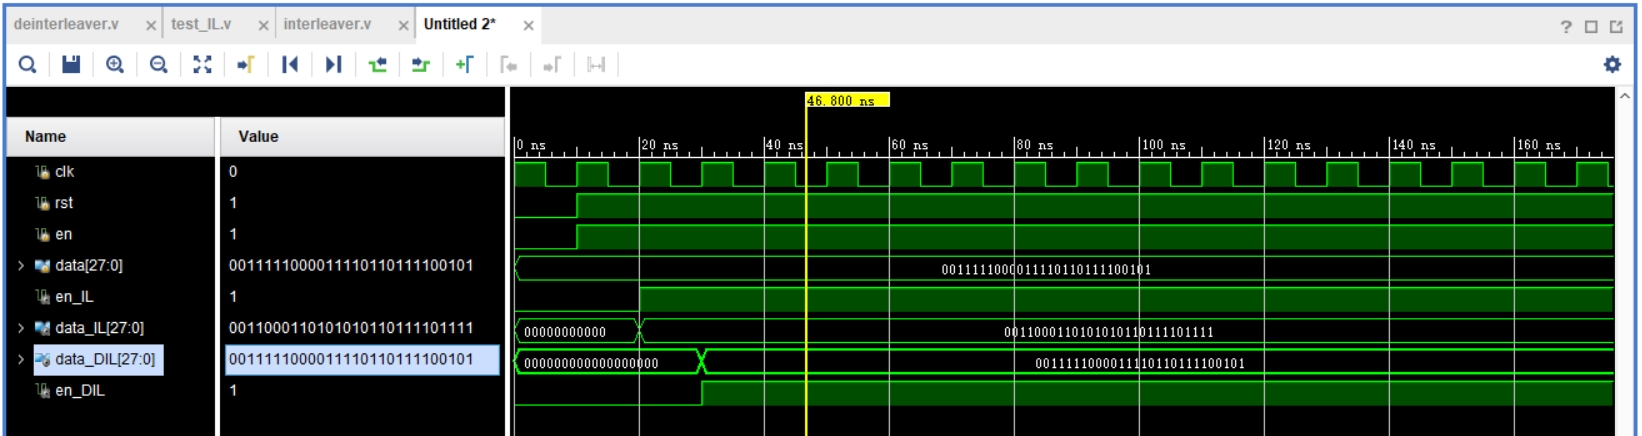
\includegraphics[width=1.0\textwidth]{static/interleave.png}
    \caption{交织与解交织仿真波形}
    \label{fig:interleave_simulation1}
\end{figure}

如图 \ref{fig:interleave_simulation2} 所示,按照“按行写入,按列读出”这一规则处理输入序列 0011111 0000111 1011011 1100101,得到的交织器输出序列应为 0011000 1101010 1011011 1101111,与图 \ref{fig:interleave_simulation1} 中的data\_IL 波形一致,说明交织器设计正确,且data\_DIL 和输入序列 data 相同,说明解交织器设计正确。

\begin{figure}[ht]
    \centering
    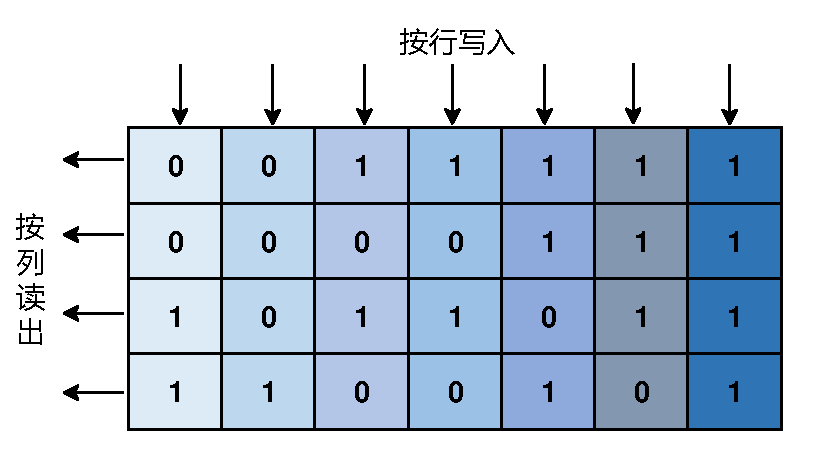
\includegraphics[width=.7\textwidth]{static/interleave_simulation.pdf}
    \caption{交织过程演示}
    \label{fig:interleave_simulation2}
\end{figure}

\subsection{QPSK 调制解调}

仿真文件如下:
\begin{codeblock}{verilog}
module test();
    parameter clk_period_100M = 10; // f=100MHz <=> T=10ns
    reg rst;
    reg clk;
    reg [15:0] datas = 16'b1110110110001101;
    wire [1:0] data_i;
    assign data_i = datas[1:0];
    wire signed [15:0] data_o_i;
    wire signed [15:0] data_o_q;
    qpsk_modulator qpsk_modulator_0 (
        .clk(clk),
        .rst(rst),
        .data_i(data_i),
        .data_o_i(data_o_i),
        .data_o_q(data_o_q)
    );
    wire [1:0] data_o;
    qpsk_demodulator qpsk_demodulator_0 (
        .clk(clk),
        .rst(rst),
        .data_i_i(data_o_i),
        .data_i_q(data_o_q),
        .data_o(data_o)
    );
    initial begin
        rst <= 0;
        clk <= 1;
        #(clk_period_100M) rst <= 1;
        #(clk_period_100M/2)
        while (datas > 0) begin
            datas <= datas >> 2;
            #(clk_period_100M) ;
        end
    end
    always #(clk_period_100M/2) clk <= ~clk;
endmodule
\end{codeblock}

仿真结果如图 \ref{fig:qpsk_simulation} 所示。

\begin{figure}[ht]
    \centering
    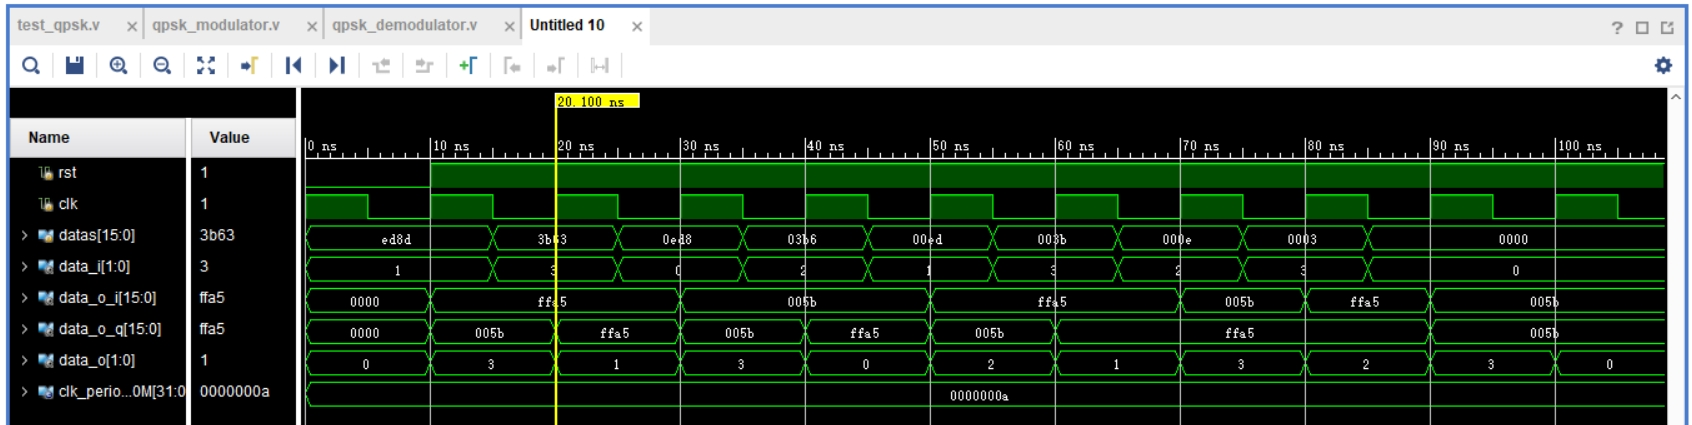
\includegraphics[width=1.0\textwidth]{static/qpsk.png}
    \caption{QPSK 调制解调器仿真波形}
    \label{fig:qpsk_simulation}
\end{figure}

从第三个时钟周期开始,每个时钟周期的 QPSK 解调器的输出 data\_o 都与前一个时钟周期的 QPSK 调制器的输入 data\_i 相等,这说明 QPSK 调制/解调器的设计正确。

\subsection{AWGN 信道模型}

我们保存了仿真产生的高斯白噪声数值,并进行了正态分布假设检验

\begin{codeblock}{verilog}
integer log_file;
initial log_file = \$fopen("simulation_log.txt", "w");
always @(posedge clk) begin
    \$fwrite(log_file, "%d\n", gaussian_noise_channel_0.gaussian_o_0);
    \$fflush(log_file);
end
\end{codeblock}

得到高斯白噪声序列(1000 条),并进行正态分布检验,结果如图 \ref{fig:gaussian_simulation} 所示。可见,概率密度分布和 QQ 图均符合高斯分布的特性。


下面进行严格的正态性检验:

首先进行 Shapiro-Wilk 正态性检验,得到统计量 $W = 0.998$,$p = 0.310$,因此我们无法拒绝高斯分布的假设;同时进行 Kolmogorov-Smirnov 正态性检验,得到统计量 $D = 0.027$,$p = 0.462$,同样无法拒绝高斯分布的假设。

\begin{figure}[ht]
    \centering
    \begin{subfigure}[b]{0.48\textwidth}
        \centering
        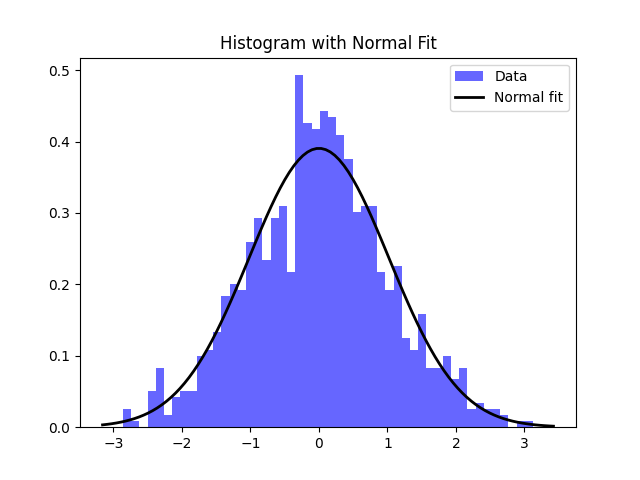
\includegraphics[width=\textwidth]{static/gaussian_fit.png}
        \caption{
            高斯白噪声概率密度分布可视化
        }\label{fig:gaussian_fit}
    \end{subfigure}
    \hfill
    \begin{subfigure}[b]{0.48\textwidth}
        \centering
        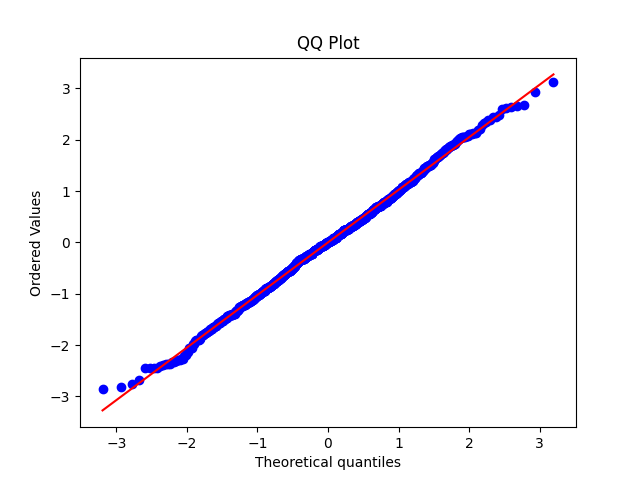
\includegraphics[width=\textwidth]{static/gaussian_qq.png}
        \caption{
            高斯白噪声 QQ 图
        }\label{fig:gaussian_qq}
    \end{subfigure}
    \caption{
        高斯白噪声分布检验
    }\label{fig:gaussian_simulation}
\end{figure}

最后检验自相关性,如图 \ref{fig:gaussian_acf} 所示,分别取 lag 为 20 和 40,自相关性函数均在 0 附近波动,且绝大部分位于 95\% 置信区间内,因此我们可以认为噪声序列是独立同分布的。


\begin{figure}[ht]
    \centering
    \begin{subfigure}[b]{0.48\textwidth}
        \centering
        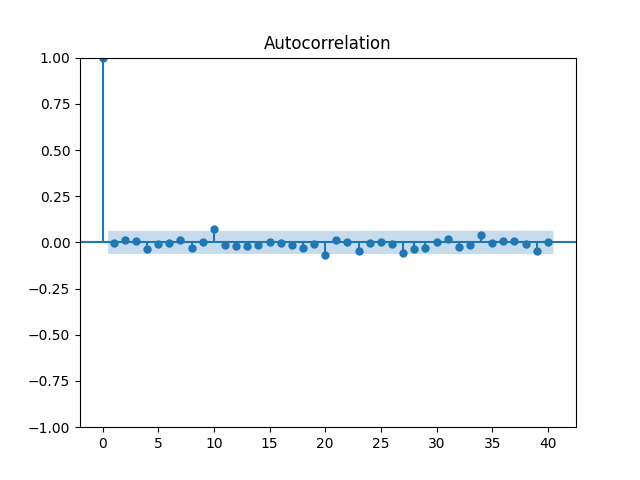
\includegraphics[width=\textwidth]{static/gaussian_acf_40.png}
        \caption{
            高斯白噪声 ACF(lag=40)
        }\label{fig:gaussian_acf_40}
    \end{subfigure}
    \hfill
    \begin{subfigure}[b]{0.48\textwidth}
        \centering
        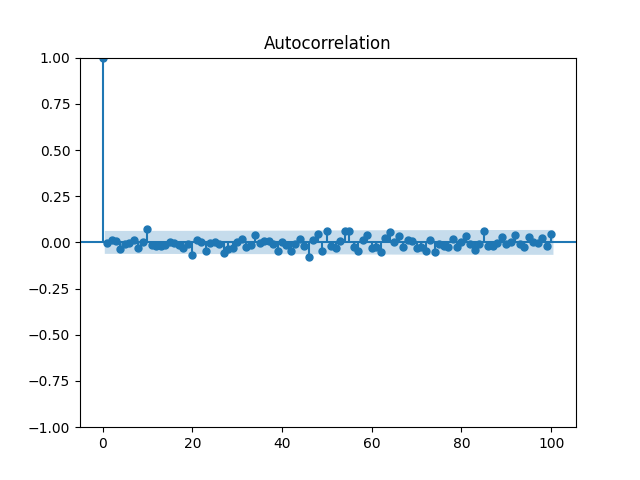
\includegraphics[width=\textwidth]{static/gaussian_acf_100.png}
        \caption{
            高斯白噪声 ACF(lag=100)
        }\label{fig:gaussian_acf_100}
    \end{subfigure}
    \caption{
        高斯白噪声自相关性检验
    }\label{fig:gaussian_acf}
\end{figure}

\subsection{联合仿真}
仿真文件如下:
\begin{codeblock}{verilog}
module test_top();
    reg clk_origin;
    reg rst;
    reg [15:0] button;
    wire [15:0] hamming_dec;
    wire hamming_wave;
    wire interres_wave;
    initial begin
        clk_origin <= 1;
        button <= 16'b0001_0100_0111_1100;
        rst <= 0;
        #5
        rst <= 1;
    end
    always #10 clk_origin = ~clk_origin;
    top top_0 (
        .clk_origin(clk_origin),
        .rst(rst),
        .button(button),
        .hamming_dec(hamming_dec),
        .hamming_wave(hamming_wave),
        .interres_wave(interres_wave)
    );
endmodule
\end{codeblock}

仿真结果如图 \ref{fig:top_simulation1} 所示。

\begin{figure}[ht]
    \centering
    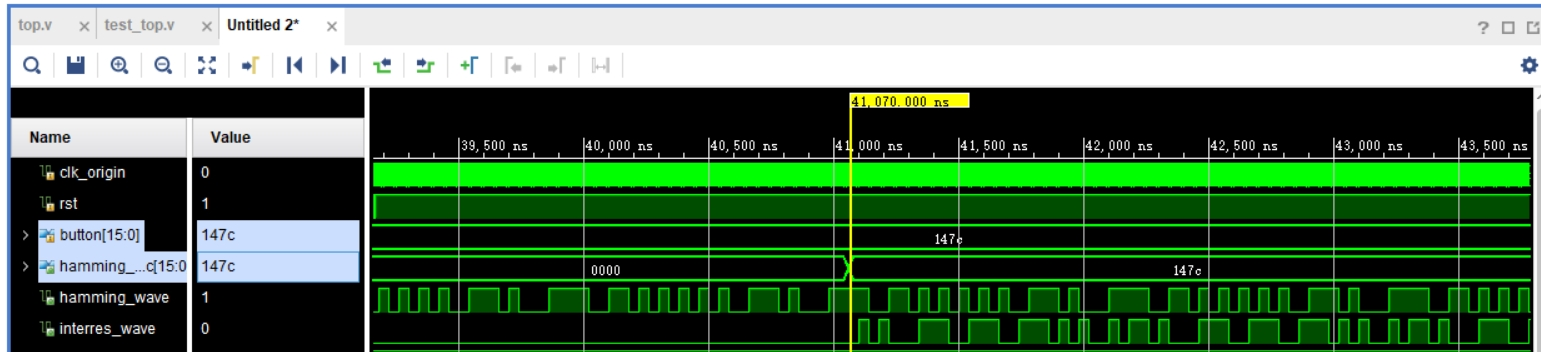
\includegraphics[width=1.0\textwidth]{static/top1.png}
    \caption{联合仿真波形}
    \label{fig:top_simulation1}
\end{figure}

读图可知,系统最终的输出 hamming\_dec 与输入 button 一致,说明系统实现正确。